\documentclass[30pt]{article}
\usepackage{geometry}
\usepackage{amsmath}
\usepackage{graphicx}
\usepackage{hyperref}

\geometry{
	a4paper,
	total={170mm,257mm},
	left=10mm, right = 10mm,
	top=15mm, bottom = 15mm,
}

\title{SVM}
\begin{document}
{\parindent0pt

{\Large \textbf{Support Vector Machine (SVM)} }

SVM support vector machine. It's similar to logistic regression but with few
changes It's said that sometimes cleaner and more powerful than other algorithms (aledgedly).

We first will start off with the hypothesis first.

Hypothesis of the Support Vector Machine is not
interpreted as the probability of y being 1 or 0 (as it is for the hypothesis
of logistic regression). Instead, it outputs either 1 or 0. (In technical
terms, it is a discriminant function.)

\section{Hypothesis}
In short No more X's, but changed into kernel. Features into kernels. That means that,
instead of $h_{\theta}(X) = g(\theta^T X)$. X's replace with kernel. that's with 
F is a vector's of f's:

\begin{equation}
	h_\theta(X)  = \theta^T*F
\end{equation}

And this $h_{\theta}(X)$ will be

\[
	h_{\theta}(X) = \left.
	\begin{cases}
		1,  & \text{for } \theta^TF \geq 0 \\
		0,  & \text{for } 0 \text{ otherwise}
	\end{cases}
	\right.
\]

\section{Kernel:Linear, gaussian kernel}

What is kernel ? Kernel is a way of selecting features for classfication problems, that's
anotherway of trying to fit a function around a data sets. Instead of polynomials, it's
using kernels to define the similarity between x and a point that they call landmark.
And in practice, people have like alot of others kerels to use. 

\textit{Note}: not all similarity functions are valid kernels. They must satisfy "Mercer's Theorem" which guarantees that the SVM package's optimizations run correctly and do not diverge.

Kernel function/similarity functions denoted: $$k(x_1,x_2)$$

The most widely used kernels are linear(Not using any kernels which is
$h_{\theta}(X)=\theta^TX$ and gaussian kernel.

The \textbf{gaussian kernel} is define:\\
X: data with m observations\\
L: land marks\\

\begin{equation}
	\text{Guassian kernel } = k(X,L) = exp(-\frac{(X - L)^2}{2\sigma^2})
\end{equation}

We then define now, our features and F vectors of f's to be:

$$f_1 = k(x,l^{(1)}), f_2 = k(x,l^{(2)}) ..., f_m = k(x,l^{(m)})$$

Or this can also be written as:

$$f_i = similarity(x,l^{(i)}) = exp(-\frac{\sum_{j=1}^{n} (x_j - l_{j}^{(i)})^2}{2\sigma^2})$$

This will have our hypothesis to look like this with m observations from X:

$$h_{\theta}(X) = \theta_0*f_0 + \theta_1*f_1 + ... + \theta_m*f_m = \theta^T*F$$

Couple of properties of these is if:

$$x \sim l^{(i)}$$ then $$f_i = exp(-\frac{\sim 0^2}{2\sigma^2}) \sim 1$$

And if 

$$x \neq l^{(i)}$$ then $$f_i = exp(-\frac{\text{Large fking number}}{2\sigma^2}) \sim 0
$$

To get predictions, plugs in X to calculates F then do a vector
inner product of $h_{\theta}(X) = \theta^TF$. If it's larger than 0, it's 1, less than 0.It's 0

*I can hear you screaming. But how the fuck does changing from polynomials into a kernel
"features" Will give out a hypothesis that will sensbily fits our function ? 

(This shit I dont' know, get on this).*

\underline{\textbf{Choosing landmarks}}:\\
One way to get the landmarks is to put them in the exact same locations as all
the training examples. This gives us m landmarks, with one landmark per
training example.

By calculating the differences some will equal to 1 some will equal to zeros. Then
from that you can draw a boundary lines around those (I think, I'm not so sure here).

\underline{sigma in gaussian kernel}:\\
$\sigma^2$ is a parameter of the Gaussian Kernel, and it can be modified to
increase or decrease the drop-off of our feature $f_i$. Combined with
looking at the values inside $\theta$, we can choose these landmarks to get the
general shape of the decision boundary.

\underline{Other algorightm application}
Using kernels to generate $f_i$'s is not exclusive to SVMs and may also be applied
to logistic regression. However, because of computational optimizations on
SVMs, kernels combined with SVMs is much faster than with other algorithms, so
kernels are almost always found combined only with SVMs.

\section{Cost function}
Similar to logistic regresision this now will have the cost when y = 0 , and y = 1 
changed to this, this is also called a Hinge loss function: \\
With $z = \theta^TF$

When y = 1
\begin{equation}
	\text{cost}_1 = max(0,\text{k}(1 - z))
\end{equation}

When y = 0
\begin{equation}
	\text{cost}_0 = max(0,\text{k}(1 + z))
\end{equation}

In general we can combine it and we will have J

\begin{multline}
	J(\theta) = C[\sum_{i=1}^{m} y^{(i)}\text{cost}_1(\theta^Tf^{(i)}) + (1 - y^{(i)})\text{cost}_0(\theta^Tf^{(i)})] + \frac{1}{2} \sum_{j=1}^m \theta_j ^ 2\\
	= C [y^T \text{cost}_1(z) + (1 - y)^T \text{cost}_0(z)] + \frac{1}{2} \sum_{j=1}^m \theta_j ^ 2
\end{multline}

graphs on $\text{cost}_0$ and $\text{cost}_1$ in magenta line, blue line is cost
of logistic regression

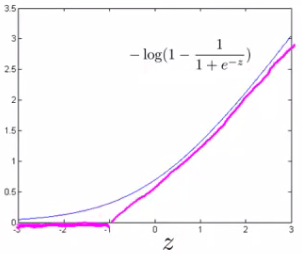
\includegraphics[scale=0.9]{cost_0.png}

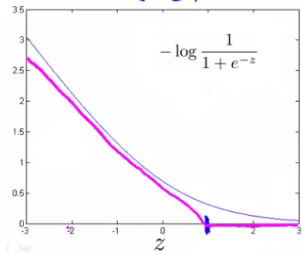
\includegraphics[scale=0.9]{cost_1.png}

As you can see, if y = 1 and $\theta^TF$ is larger than 1, the cost is 0.
And, if y = 0 and $\theta^TF$ is less than -1, the cost is 0. Otherwise it's additioning
the line with k as an abitrary number.

This is also the reason why the SVM is sometimes called the large margin classifer.
Lies in the vector inner product, to understand further on why it's called a large
margin classifer. Watch Mr andrew Ng video again on week 7 coursera on why it's 
called a largemargin classifer.

\section{Implementation}
Now, Professor Andrew Ng doesn't mention what we are using to optimized this, but instead
he points to an off the shelf library. That people have already optimized the shit
out of. You just need to use, Don't worry about the details. But when using 
the library he suggests a some listed here:

\url{https://www.csie.ntu.edu.tw/~cjlin/liblinear/}\\
\url{https://www.csie.ntu.edu.tw/~cjlin/libsvm/}

To evaluates which C or sigma, he suggests we check out the lowest error in cross
validation set.

A few C's and sigma's to try out. Test each C with each sigma for best effect
Below are the octave code

\begin{verbatim}
C_vec = [0.01, 0.03, 0.1, 0.3, 1, 3, 10, 30];
sigma_vec = [0.01, 0.03, 0.1, 0.3, 1, 3, 10, 30];
\end{verbatim}

Error cross validation is 

\begin{verbatim}
	error_cv = mean(double(predictions ~= y));
\end{verbatim}

Bias and variacne controlling with C and sigma

\textbf{C}
\begin{itemize}
	\item C large: Lower bias, high variacne
	\item C small: High bias, low variacne.
\end{itemize}

\textbf{sigma}
\begin{itemize}
	\item sigma large: Feature $f_i$, vary more smoothly, Higher bias, lower variacne.
	\item sigma small: Feature $f_i$, vary less smoothly, Lower bias, higher variacne.
\end{itemize}

\section{Using SVM library}

When using SVM library here are the list of things that you need to provide to 
the algorithm :

\begin{itemize}
	\item Choice of kernel (Linear kernel y = 1 if $\theta^Tx \geq 0$) or gaussian
		(And be sure it's satisfied Mercer's theorm)
	\item Choice of C
\end{itemize}

If you choose gaussian kernel, prepare gaussian kernel as gaussian($x_1,x_2$) then

\begin{itemize}
	\item Choice of $\sigma$
	\item Perform feature scaling (Read on this if needed) Really needed, if not
		shit will not work as advertised
\end{itemize}

Professor said that he doesn't used alot of other kernels but here they are:
polynomial kernel, string kernel, chi-square kernel, histogram kernel, 	intersection
kernel,...

\section{Multiclassification}

If your library doesn't have multiclassification purpose, just 1vsall. let y = to each
group. If there are 3 group, then to get $\theta$ for group 1 let y = 1 if y = group 1
and let y = 0 if y $\neq$ group 1. Do that for for all 3 groups, then we should have
3 $\theta$'s for 3 group.

\section{SVM or Logistic regression ? Cons, pros}

Okay, so when should we use logistic regression ? and when should we use SVM ?

n = numbers of features ($x \in R^{n+1}$), m = numbers of observations 

\underline{Case} \#1:
n is large (relative to m): $n \geq m$, n = 10,000 , m = 10,...,1000)\\
\textbf{Use}:
Logistic regression, or SVM without a kernel("linear kernel")

\underline{Case}\#2:
n is small, m is intermediate (n = 1...1000, m = 10,...,10,000)\\
\textbf{Use}: 
SVM with gaussian kernel

\underline{Case} \#3:
n is small, m is large\\
\textbf{Use}:
Create/add more features, then use logistic regression or SVM without a kernel

Neural network will likely to work for all of these, but takes more time to train.

\section{Additional reference}
\url{https://web.mit.edu/6.034/wwwbob/svm-notes-long-08.pdf}
\end{document}
